\documentclass[1p]{elsarticle_modified}
%\bibliographystyle{elsarticle-num}

%\usepackage[colorlinks]{hyperref}
%\usepackage{abbrmath_seonhwa} %\Abb, \Ascr, \Acal ,\Abf, \Afrak
\usepackage{amsfonts}
\usepackage{amssymb}
\usepackage{amsmath}
\usepackage{amsthm}
\usepackage{scalefnt}
\usepackage{amsbsy}
\usepackage{kotex}
\usepackage{caption}
\usepackage{subfig}
\usepackage{color}
\usepackage{graphicx}
\usepackage{xcolor} %% white, black, red, green, blue, cyan, magenta, yellow
\usepackage{float}
\usepackage{setspace}
\usepackage{hyperref}

\usepackage{tikz}
\usetikzlibrary{arrows}

\usepackage{multirow}
\usepackage{array} % fixed length table
\usepackage{hhline}

%%%%%%%%%%%%%%%%%%%%%
\makeatletter
\renewcommand*\env@matrix[1][\arraystretch]{%
	\edef\arraystretch{#1}%
	\hskip -\arraycolsep
	\let\@ifnextchar\new@ifnextchar
	\array{*\c@MaxMatrixCols c}}
\makeatother %https://tex.stackexchange.com/questions/14071/how-can-i-increase-the-line-spacing-in-a-matrix
%%%%%%%%%%%%%%%

\usepackage[normalem]{ulem}

\newcommand{\msout}[1]{\ifmmode\text{\sout{\ensuremath{#1}}}\else\sout{#1}\fi}
%SOURCE: \msout is \stkout macro in https://tex.stackexchange.com/questions/20609/strikeout-in-math-mode

\newcommand{\cancel}[1]{
	\ifmmode
	{\color{red}\msout{#1}}
	\else
	{\color{red}\sout{#1}}
	\fi
}

\newcommand{\add}[1]{
	{\color{blue}\uwave{#1}}
}

\newcommand{\replace}[2]{
	\ifmmode
	{\color{red}\msout{#1}}{\color{blue}\uwave{#2}}
	\else
	{\color{red}\sout{#1}}{\color{blue}\uwave{#2}}
	\fi
}

\newcommand{\Sol}{\mathcal{S}} %segment
\newcommand{\D}{D} %diagram
\newcommand{\A}{\mathcal{A}} %arc


%%%%%%%%%%%%%%%%%%%%%%%%%%%%%5 test

\def\sl{\operatorname{\textup{SL}}(2,\Cbb)}
\def\psl{\operatorname{\textup{PSL}}(2,\Cbb)}
\def\quan{\mkern 1mu \triangleright \mkern 1mu}

\theoremstyle{definition}
\newtheorem{thm}{Theorem}[section]
\newtheorem{prop}[thm]{Proposition}
\newtheorem{lem}[thm]{Lemma}
\newtheorem{ques}[thm]{Question}
\newtheorem{cor}[thm]{Corollary}
\newtheorem{defn}[thm]{Definition}
\newtheorem{exam}[thm]{Example}
\newtheorem{rmk}[thm]{Remark}
\newtheorem{alg}[thm]{Algorithm}

\newcommand{\I}{\sqrt{-1}}
\begin{document}

%\begin{frontmatter}
%
%\title{Boundary parabolic representations of knots up to 8 crossings}
%
%%% Group authors per affiliation:
%\author{Yunhi Cho} 
%\address{Department of Mathematics, University of Seoul, Seoul, Korea}
%\ead{yhcho@uos.ac.kr}
%
%
%\author{Seonhwa Kim} %\fnref{s_kim}}
%\address{Center for Geometry and Physics, Institute for Basic Science, Pohang, 37673, Korea}
%\ead{ryeona17@ibs.re.kr}
%
%\author{Hyuk Kim}
%\address{Department of Mathematical Sciences, Seoul National University, Seoul 08826, Korea}
%\ead{hyukkim@snu.ac.kr}
%
%\author{Seokbeom Yoon}
%\address{Department of Mathematical Sciences, Seoul National University, Seoul, 08826,  Korea}
%\ead{sbyoon15@snu.ac.kr}
%
%\begin{abstract}
%We find all boundary parabolic representation of knots up to 8 crossings.
%
%\end{abstract}
%\begin{keyword}
%    \MSC[2010] 57M25 
%\end{keyword}
%
%\end{frontmatter}

%\linenumbers
%\tableofcontents
%
\newcommand\colored[1]{\textcolor{white}{\rule[-0.35ex]{0.8em}{1.4ex}}\kern-0.8em\color{red} #1}%
%\newcommand\colored[1]{\textcolor{white}{ #1}\kern-2.17ex	\textcolor{white}{ #1}\kern-1.81ex	\textcolor{white}{ #1}\kern-2.15ex\color{red}#1	}

{\Large $\underline{12n_{0105}~(K12n_{0105})}$}

\setlength{\tabcolsep}{10pt}
\renewcommand{\arraystretch}{1.6}
\vspace{1cm}\begin{tabular}{m{100pt}>{\centering\arraybackslash}m{274pt}}
\multirow{5}{120pt}{
	\centering
	\includegraphics[width=112pt]{../../../GIT/diagram.site/Diagrams/png/2194_12n_0105.png}\\
\ \ \ A knot diagram\footnotemark}&
\allowdisplaybreaks
\textbf{Linearized knot diagam} \\
\cline{2-2}
 &
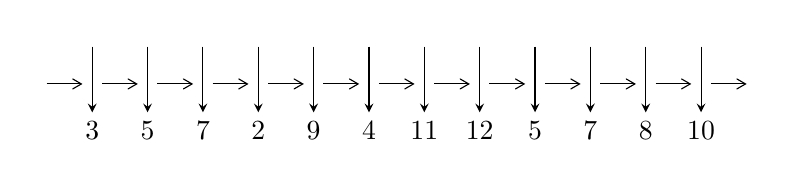
\begin{tikzpicture}[x=20pt, y=17pt]
	% nodes
	\node (C0) at (0, 0) {};
	\node (C1) at (1, 0) {};
	\node (C1U) at (1, +1) {};
	\node (C1D) at (1, -1) {3};

	\node (C2) at (2, 0) {};
	\node (C2U) at (2, +1) {};
	\node (C2D) at (2, -1) {5};

	\node (C3) at (3, 0) {};
	\node (C3U) at (3, +1) {};
	\node (C3D) at (3, -1) {7};

	\node (C4) at (4, 0) {};
	\node (C4U) at (4, +1) {};
	\node (C4D) at (4, -1) {2};

	\node (C5) at (5, 0) {};
	\node (C5U) at (5, +1) {};
	\node (C5D) at (5, -1) {9};

	\node (C6) at (6, 0) {};
	\node (C6U) at (6, +1) {};
	\node (C6D) at (6, -1) {4};

	\node (C7) at (7, 0) {};
	\node (C7U) at (7, +1) {};
	\node (C7D) at (7, -1) {11};

	\node (C8) at (8, 0) {};
	\node (C8U) at (8, +1) {};
	\node (C8D) at (8, -1) {12};

	\node (C9) at (9, 0) {};
	\node (C9U) at (9, +1) {};
	\node (C9D) at (9, -1) {5};

	\node (C10) at (10, 0) {};
	\node (C10U) at (10, +1) {};
	\node (C10D) at (10, -1) {7};

	\node (C11) at (11, 0) {};
	\node (C11U) at (11, +1) {};
	\node (C11D) at (11, -1) {8};

	\node (C12) at (12, 0) {};
	\node (C12U) at (12, +1) {};
	\node (C12D) at (12, -1) {10};
	\node (C13) at (13, 0) {};

	% arrows
	\draw[->,>={angle 60}]
	(C0) edge (C1) (C1) edge (C2) (C2) edge (C3) (C3) edge (C4) (C4) edge (C5) (C5) edge (C6) (C6) edge (C7) (C7) edge (C8) (C8) edge (C9) (C9) edge (C10) (C10) edge (C11) (C11) edge (C12) (C12) edge (C13) ;	\draw[->,>=stealth]
	(C1U) edge (C1D) (C2U) edge (C2D) (C3U) edge (C3D) (C4U) edge (C4D) (C5U) edge (C5D) (C6U) edge (C6D) (C7U) edge (C7D) (C8U) edge (C8D) (C9U) edge (C9D) (C10U) edge (C10D) (C11U) edge (C11D) (C12U) edge (C12D) ;
	\end{tikzpicture} \\
\hhline{~~} \\& 
\textbf{Solving Sequence} \\ \cline{2-2} 
 &
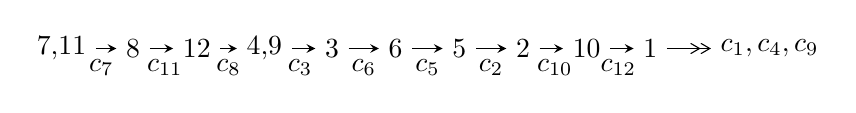
\begin{tikzpicture}[x=23pt, y=7pt]
	% node
	\node (A0) at (-1/8, 0) {7,11};
	\node (A1) at (1, 0) {8};
	\node (A2) at (2, 0) {12};
	\node (A3) at (49/16, 0) {4,9};
	\node (A4) at (33/8, 0) {3};
	\node (A5) at (41/8, 0) {6};
	\node (A6) at (49/8, 0) {5};
	\node (A7) at (57/8, 0) {2};
	\node (A8) at (65/8, 0) {10};
	\node (A9) at (73/8, 0) {1};
	\node (C1) at (1/2, -1) {$c_{7}$};
	\node (C2) at (3/2, -1) {$c_{11}$};
	\node (C3) at (5/2, -1) {$c_{8}$};
	\node (C4) at (29/8, -1) {$c_{3}$};
	\node (C5) at (37/8, -1) {$c_{6}$};
	\node (C6) at (45/8, -1) {$c_{5}$};
	\node (C7) at (53/8, -1) {$c_{2}$};
	\node (C8) at (61/8, -1) {$c_{10}$};
	\node (C9) at (69/8, -1) {$c_{12}$};
	\node (A10) at (11, 0) {$c_{1},c_{4},c_{9}$};

	% edge
	\draw[->,>=stealth]	
	(A0) edge (A1) (A1) edge (A2) (A2) edge (A3) (A3) edge (A4) (A4) edge (A5) (A5) edge (A6) (A6) edge (A7) (A7) edge (A8) (A8) edge (A9) ;
	\draw[->>,>={angle 60}]	
	(A9) edge (A10);
\end{tikzpicture} \\ 

\end{tabular} \\

\footnotetext{
The image of knot diagram is generated by the software ``\textbf{Draw programme}" developed by Andrew Bartholomew(\url{http://www.layer8.co.uk/maths/draw/index.htm\#Running-draw}), where we modified some parts for our purpose(\url{https://github.com/CATsTAILs/LinksPainter}).
}\phantom \\ \newline 
\centering \textbf{Ideals for irreducible components\footnotemark of $X_{\text{par}}$} 
 
\begin{align*}
I^u_{1}&=\langle 
22873134 u^{26}-91748515 u^{25}+\cdots+37746988 b-44822939,\\
\phantom{I^u_{1}}&\phantom{= \langle  }63338341 u^{26}-295194910 u^{25}+\cdots+37746988 a-66189548,\;u^{27}-5 u^{26}+\cdots-6 u+1\rangle \\
I^u_{2}&=\langle 
b,\;2 u^5- u^4-7 u^3+u^2+a+5 u+4,\;u^6- u^5-3 u^4+2 u^3+2 u^2+u-1\rangle \\
I^u_{3}&=\langle 
- a^2+b-3 a-1,\;a^3+3 a^2+2 a+1,\;u^2+u-1\rangle \\
\\
\end{align*}
\raggedright * 3 irreducible components of $\dim_{\mathbb{C}}=0$, with total 39 representations.\\
\footnotetext{All coefficients of polynomials are rational numbers. But the coefficients are sometimes approximated in decimal forms when there is not enough margin.}
\newpage
\renewcommand{\arraystretch}{1}
\centering \section*{I. $I^u_{1}= \langle 2.29\times10^{7} u^{26}-9.17\times10^{7} u^{25}+\cdots+3.77\times10^{7} b-4.48\times10^{7},\;6.33\times10^{7} u^{26}-2.95\times10^{8} u^{25}+\cdots+3.77\times10^{7} a-6.62\times10^{7},\;u^{27}-5 u^{26}+\cdots-6 u+1 \rangle$}
\flushleft \textbf{(i) Arc colorings}\\
\begin{tabular}{m{7pt} m{180pt} m{7pt} m{180pt} }
\flushright $a_{7}=$&$\begin{pmatrix}1\\0\end{pmatrix}$ \\
\flushright $a_{11}=$&$\begin{pmatrix}0\\u\end{pmatrix}$ \\
\flushright $a_{8}=$&$\begin{pmatrix}1\\u^2\end{pmatrix}$ \\
\flushright $a_{12}=$&$\begin{pmatrix}- u\\- u^3+u\end{pmatrix}$ \\
\flushright $a_{4}=$&$\begin{pmatrix}-1.67797 u^{26}+7.82036 u^{25}+\cdots-8.45077 u+1.75351\\-0.605959 u^{26}+2.43062 u^{25}+\cdots-2.79918 u+1.18746\end{pmatrix}$ \\
\flushright $a_{9}=$&$\begin{pmatrix}- u^2+1\\- u^4+2 u^2\end{pmatrix}$ \\
\flushright $a_{3}=$&$\begin{pmatrix}-2.28393 u^{26}+10.2510 u^{25}+\cdots-11.2499 u+2.94096\\-0.605959 u^{26}+2.43062 u^{25}+\cdots-2.79918 u+1.18746\end{pmatrix}$ \\
\flushright $a_{6}=$&$\begin{pmatrix}-0.101693 u^{26}+0.926944 u^{25}+\cdots-7.17642 u+3.14845\\1.45363 u^{26}-5.69060 u^{25}+\cdots+5.80702 u-1.50691\end{pmatrix}$ \\
\flushright $a_{5}=$&$\begin{pmatrix}0.758454 u^{26}-2.47127 u^{25}+\cdots-3.68028 u+1.91598\\0.144041 u^{26}-0.819382 u^{25}+\cdots+0.700822 u-0.562543\end{pmatrix}$ \\
\flushright $a_{2}=$&$\begin{pmatrix}-1.05084 u^{26}+5.94352 u^{25}+\cdots-11.3894 u+3.35900\\-0.144041 u^{26}+0.819382 u^{25}+\cdots-0.700822 u+0.562543\end{pmatrix}$ \\
\flushright $a_{10}=$&$\begin{pmatrix}u\\u\end{pmatrix}$ \\
\flushright $a_{1}=$&$\begin{pmatrix}u^5-2 u^3- u\\u^5-3 u^3+u\end{pmatrix}$\\&\end{tabular}
\flushleft \textbf{(ii) Obstruction class $= -1$}\\~\\
\flushleft \textbf{(iii) Cusp Shapes $= -\frac{725958293}{18873494} u^{26}+\frac{3202886145}{18873494} u^{25}+\cdots-\frac{5326606613}{18873494} u+\frac{1076937225}{18873494}$}\\~\\
\newpage\renewcommand{\arraystretch}{1}
\flushleft \textbf{(iv) u-Polynomials at the component}\newline \\
\begin{tabular}{m{50pt}|m{274pt}}
Crossings & \hspace{64pt}u-Polynomials at each crossing \\
\hline $$\begin{aligned}c_{1}\end{aligned}$$&$\begin{aligned}
&u^{27}+u^{26}+\cdots+514 u+1
\end{aligned}$\\
\hline $$\begin{aligned}c_{2},c_{4}\end{aligned}$$&$\begin{aligned}
&u^{27}-9 u^{26}+\cdots+20 u+1
\end{aligned}$\\
\hline $$\begin{aligned}c_{3},c_{6}\end{aligned}$$&$\begin{aligned}
&u^{27}-3 u^{26}+\cdots+128 u+64
\end{aligned}$\\
\hline $$\begin{aligned}c_{5},c_{9}\end{aligned}$$&$\begin{aligned}
&u^{27}+2 u^{26}+\cdots-352 u-64
\end{aligned}$\\
\hline $$\begin{aligned}c_{7},c_{8},c_{10}\\c_{11}\end{aligned}$$&$\begin{aligned}
&u^{27}+5 u^{26}+\cdots-6 u-1
\end{aligned}$\\
\hline $$\begin{aligned}c_{12}\end{aligned}$$&$\begin{aligned}
&u^{27}+u^{26}+\cdots+500 u-89
\end{aligned}$\\
\hline
\end{tabular}\\~\\
\newpage\renewcommand{\arraystretch}{1}
\flushleft \textbf{(v) Riley Polynomials at the component}\newline \\
\begin{tabular}{m{50pt}|m{274pt}}
Crossings & \hspace{64pt}Riley Polynomials at each crossing \\
\hline $$\begin{aligned}c_{1}\end{aligned}$$&$\begin{aligned}
&y^{27}+59 y^{26}+\cdots+262978 y-1
\end{aligned}$\\
\hline $$\begin{aligned}c_{2},c_{4}\end{aligned}$$&$\begin{aligned}
&y^{27}- y^{26}+\cdots+514 y-1
\end{aligned}$\\
\hline $$\begin{aligned}c_{3},c_{6}\end{aligned}$$&$\begin{aligned}
&y^{27}+45 y^{26}+\cdots+180224 y-4096
\end{aligned}$\\
\hline $$\begin{aligned}c_{5},c_{9}\end{aligned}$$&$\begin{aligned}
&y^{27}+40 y^{26}+\cdots+103424 y-4096
\end{aligned}$\\
\hline $$\begin{aligned}c_{7},c_{8},c_{10}\\c_{11}\end{aligned}$$&$\begin{aligned}
&y^{27}-29 y^{26}+\cdots-14 y-1
\end{aligned}$\\
\hline $$\begin{aligned}c_{12}\end{aligned}$$&$\begin{aligned}
&y^{27}+67 y^{26}+\cdots-314794 y-7921
\end{aligned}$\\
\hline
\end{tabular}\\~\\
\newpage\flushleft \textbf{(vi) Complex Volumes and Cusp Shapes}
$$\begin{array}{c|c|c}  
\text{Solutions to }I^u_{1}& \I (\text{vol} + \sqrt{-1}CS) & \text{Cusp shape}\\
 \hline 
\begin{aligned}
u &= -0.514269 + 0.943772 I \\
a &= \phantom{-}0.96114 + 1.49139 I \\
b &= -0.33697 - 2.32589 I\end{aligned}
 & \phantom{-}15.0681 - 1.4972 I & -9.94344 - 0.11775 I \\ \hline\begin{aligned}
u &= -0.514269 - 0.943772 I \\
a &= \phantom{-}0.96114 - 1.49139 I \\
b &= -0.33697 + 2.32589 I\end{aligned}
 & \phantom{-}15.0681 + 1.4972 I & -9.94344 + 0.11775 I \\ \hline\begin{aligned}
u &= -0.664233 + 0.874955 I \\
a &= -1.06704 - 1.64357 I \\
b &= -0.62816 + 2.16426 I\end{aligned}
 & \phantom{-}14.6013 + 7.4637 I & -10.63048 - 4.31713 I \\ \hline\begin{aligned}
u &= -0.664233 - 0.874955 I \\
a &= -1.06704 + 1.64357 I \\
b &= -0.62816 - 2.16426 I\end{aligned}
 & \phantom{-}14.6013 - 7.4637 I & -10.63048 + 4.31713 I \\ \hline\begin{aligned}
u &= -1.182480 + 0.163891 I \\
a &= \phantom{-}0.485579 + 0.426627 I \\
b &= \phantom{-}0.14520 - 1.74397 I\end{aligned}
 & \phantom{-}1.12392 + 3.54626 I & -14.5183 - 3.2040 I \\ \hline\begin{aligned}
u &= -1.182480 - 0.163891 I \\
a &= \phantom{-}0.485579 - 0.426627 I \\
b &= \phantom{-}0.14520 + 1.74397 I\end{aligned}
 & \phantom{-}1.12392 - 3.54626 I & -14.5183 + 3.2040 I \\ \hline\begin{aligned}
u &= \phantom{-}1.261340 + 0.096236 I \\
a &= \phantom{-}0.969318 + 0.141624 I \\
b &= \phantom{-}0.808086 - 0.842084 I\end{aligned}
 & -4.50481 - 1.41612 I & -14.8457 + 0.7290 I \\ \hline\begin{aligned}
u &= \phantom{-}1.261340 - 0.096236 I \\
a &= \phantom{-}0.969318 - 0.141624 I \\
b &= \phantom{-}0.808086 + 0.842084 I\end{aligned}
 & -4.50481 + 1.41612 I & -14.8457 - 0.7290 I \\ \hline\begin{aligned}
u &= -0.153216 + 0.715283 I \\
a &= -0.15544 - 1.50896 I \\
b &= -0.68505 + 1.29368 I\end{aligned}
 & \phantom{-}3.93766 - 0.32566 I & -7.68828 - 0.01937 I \\ \hline\begin{aligned}
u &= -0.153216 - 0.715283 I \\
a &= -0.15544 + 1.50896 I \\
b &= -0.68505 - 1.29368 I\end{aligned}
 & \phantom{-}3.93766 + 0.32566 I & -7.68828 + 0.01937 I\\
 \hline 
 \end{array}$$\newpage$$\begin{array}{c|c|c}  
\text{Solutions to }I^u_{1}& \I (\text{vol} + \sqrt{-1}CS) & \text{Cusp shape}\\
 \hline 
\begin{aligned}
u &= -0.543053 + 0.346105 I \\
a &= \phantom{-}0.952357 - 0.112943 I \\
b &= \phantom{-}0.116929 - 1.071230 I\end{aligned}
 & \phantom{-}2.02138 + 3.53683 I & -8.00351 - 9.60393 I \\ \hline\begin{aligned}
u &= -0.543053 - 0.346105 I \\
a &= \phantom{-}0.952357 + 0.112943 I \\
b &= \phantom{-}0.116929 + 1.071230 I\end{aligned}
 & \phantom{-}2.02138 - 3.53683 I & -8.00351 + 9.60393 I \\ \hline\begin{aligned}
u &= \phantom{-}1.348160 + 0.304621 I \\
a &= -0.990189 + 0.519594 I \\
b &= -1.27433 - 0.79621 I\end{aligned}
 & -0.78811 - 3.39068 I & -12.00000 + 2.97054 I \\ \hline\begin{aligned}
u &= \phantom{-}1.348160 - 0.304621 I \\
a &= -0.990189 - 0.519594 I \\
b &= -1.27433 + 0.79621 I\end{aligned}
 & -0.78811 + 3.39068 I & -12.00000 - 2.97054 I \\ \hline\begin{aligned}
u &= \phantom{-}0.552139\phantom{ +0.000000I} \\
a &= -7.52398\phantom{ +0.000000I} \\
b &= -0.222467\phantom{ +0.000000I}\end{aligned}
 & -2.46059\phantom{ +0.000000I} & -111.160\phantom{ +0.000000I} \\ \hline\begin{aligned}
u &= \phantom{-}1.53250 + 0.12438 I \\
a &= \phantom{-}0.477076 + 0.429045 I \\
b &= \phantom{-}0.181555 + 0.768118 I\end{aligned}
 & -4.88486 - 5.37353 I & -12.0000 + 7.7726 I \\ \hline\begin{aligned}
u &= \phantom{-}1.53250 - 0.12438 I \\
a &= \phantom{-}0.477076 - 0.429045 I \\
b &= \phantom{-}0.181555 - 0.768118 I\end{aligned}
 & -4.88486 + 5.37353 I & -12.0000 - 7.7726 I \\ \hline\begin{aligned}
u &= -1.55351 + 0.07692 I \\
a &= -0.278760 + 0.128293 I \\
b &= \phantom{-}0.464875 + 0.727258 I\end{aligned}
 & -7.33821 + 0.72358 I & -12.00000 + 0. I\phantom{ +0.000000I} \\ \hline\begin{aligned}
u &= -1.55351 - 0.07692 I \\
a &= -0.278760 - 0.128293 I \\
b &= \phantom{-}0.464875 - 0.727258 I\end{aligned}
 & -7.33821 - 0.72358 I & -12.00000 + 0. I\phantom{ +0.000000I} \\ \hline\begin{aligned}
u &= \phantom{-}0.440522\phantom{ +0.000000I} \\
a &= -0.842102\phantom{ +0.000000I} \\
b &= \phantom{-}0.209937\phantom{ +0.000000I}\end{aligned}
 & -0.703245\phantom{ +0.000000I} & -13.8830\phantom{ +0.000000I}\\
 \hline 
 \end{array}$$\newpage$$\begin{array}{c|c|c}  
\text{Solutions to }I^u_{1}& \I (\text{vol} + \sqrt{-1}CS) & \text{Cusp shape}\\
 \hline 
\begin{aligned}
u &= -1.60962\phantom{ +0.000000I} \\
a &= -3.04132\phantom{ +0.000000I} \\
b &= -0.471477\phantom{ +0.000000I}\end{aligned}
 & -10.1232\phantom{ +0.000000I} & -65.7520\phantom{ +0.000000I} \\ \hline\begin{aligned}
u &= \phantom{-}1.56503 + 0.38318 I \\
a &= \phantom{-}0.979548 - 0.112812 I \\
b &= \phantom{-}0.04694 + 2.26665 I\end{aligned}
 & \phantom{-}8.39568 - 3.40964 I & -12.00000 + 0. I\phantom{ +0.000000I} \\ \hline\begin{aligned}
u &= \phantom{-}1.56503 - 0.38318 I \\
a &= \phantom{-}0.979548 + 0.112812 I \\
b &= \phantom{-}0.04694 - 2.26665 I\end{aligned}
 & \phantom{-}8.39568 + 3.40964 I & -12.00000 + 0. I\phantom{ +0.000000I} \\ \hline\begin{aligned}
u &= \phantom{-}1.61847 + 0.30353 I \\
a &= -1.37457 + 0.38272 I \\
b &= -0.75828 - 1.91136 I\end{aligned}
 & \phantom{-}7.09877 - 11.89130 I & -12.00000 + 0. I\phantom{ +0.000000I} \\ \hline\begin{aligned}
u &= \phantom{-}1.61847 - 0.30353 I \\
a &= -1.37457 - 0.38272 I \\
b &= -0.75828 + 1.91136 I\end{aligned}
 & \phantom{-}7.09877 + 11.89130 I & -12.00000 + 0. I\phantom{ +0.000000I} \\ \hline\begin{aligned}
u &= \phantom{-}0.093749 + 0.195668 I \\
a &= -1.25531 + 1.76548 I \\
b &= \phantom{-}0.661199 + 0.033436 I\end{aligned}
 & -0.945949 + 0.075456 I & -9.99859 + 1.12534 I \\ \hline\begin{aligned}
u &= \phantom{-}0.093749 - 0.195668 I \\
a &= -1.25531 - 1.76548 I \\
b &= \phantom{-}0.661199 - 0.033436 I\end{aligned}
 & -0.945949 - 0.075456 I & -9.99859 - 1.12534 I\\
 \hline 
 \end{array}$$\newpage\newpage\renewcommand{\arraystretch}{1}
\centering \section*{II. $I^u_{2}= \langle b,\;2 u^5- u^4-7 u^3+u^2+a+5 u+4,\;u^6- u^5-3 u^4+2 u^3+2 u^2+u-1 \rangle$}
\flushleft \textbf{(i) Arc colorings}\\
\begin{tabular}{m{7pt} m{180pt} m{7pt} m{180pt} }
\flushright $a_{7}=$&$\begin{pmatrix}1\\0\end{pmatrix}$ \\
\flushright $a_{11}=$&$\begin{pmatrix}0\\u\end{pmatrix}$ \\
\flushright $a_{8}=$&$\begin{pmatrix}1\\u^2\end{pmatrix}$ \\
\flushright $a_{12}=$&$\begin{pmatrix}- u\\- u^3+u\end{pmatrix}$ \\
\flushright $a_{4}=$&$\begin{pmatrix}-2 u^5+u^4+7 u^3- u^2-5 u-4\\0\end{pmatrix}$ \\
\flushright $a_{9}=$&$\begin{pmatrix}- u^2+1\\- u^4+2 u^2\end{pmatrix}$ \\
\flushright $a_{3}=$&$\begin{pmatrix}-2 u^5+u^4+7 u^3- u^2-5 u-4\\0\end{pmatrix}$ \\
\flushright $a_{6}=$&$\begin{pmatrix}1\\0\end{pmatrix}$ \\
\flushright $a_{5}=$&$\begin{pmatrix}- u^5+2 u^3+u\\- u^5+3 u^3- u\end{pmatrix}$ \\
\flushright $a_{2}=$&$\begin{pmatrix}- u^5+u^4+5 u^3- u^2-6 u-4\\u^5-3 u^3+u\end{pmatrix}$ \\
\flushright $a_{10}=$&$\begin{pmatrix}u\\u\end{pmatrix}$ \\
\flushright $a_{1}=$&$\begin{pmatrix}u^5-2 u^3- u\\u^5-3 u^3+u\end{pmatrix}$\\&\end{tabular}
\flushleft \textbf{(ii) Obstruction class $= 1$}\\~\\
\flushleft \textbf{(iii) Cusp Shapes $= 10 u^5-6 u^4-30 u^3+5 u^2+17 u+7$}\\~\\
\newpage\renewcommand{\arraystretch}{1}
\flushleft \textbf{(iv) u-Polynomials at the component}\newline \\
\begin{tabular}{m{50pt}|m{274pt}}
Crossings & \hspace{64pt}u-Polynomials at each crossing \\
\hline $$\begin{aligned}c_{1},c_{2}\end{aligned}$$&$\begin{aligned}
&(u-1)^6
\end{aligned}$\\
\hline $$\begin{aligned}c_{3},c_{6}\end{aligned}$$&$\begin{aligned}
&u^6
\end{aligned}$\\
\hline $$\begin{aligned}c_{4}\end{aligned}$$&$\begin{aligned}
&(u+1)^6
\end{aligned}$\\
\hline $$\begin{aligned}c_{5}\end{aligned}$$&$\begin{aligned}
&u^6+u^5+3 u^4+2 u^3+2 u^2+u-1
\end{aligned}$\\
\hline $$\begin{aligned}c_{7},c_{8}\end{aligned}$$&$\begin{aligned}
&u^6- u^5-3 u^4+2 u^3+2 u^2+u-1
\end{aligned}$\\
\hline $$\begin{aligned}c_{9},c_{12}\end{aligned}$$&$\begin{aligned}
&u^6- u^5+3 u^4-2 u^3+2 u^2- u-1
\end{aligned}$\\
\hline $$\begin{aligned}c_{10},c_{11}\end{aligned}$$&$\begin{aligned}
&u^6+u^5-3 u^4-2 u^3+2 u^2- u-1
\end{aligned}$\\
\hline
\end{tabular}\\~\\
\newpage\renewcommand{\arraystretch}{1}
\flushleft \textbf{(v) Riley Polynomials at the component}\newline \\
\begin{tabular}{m{50pt}|m{274pt}}
Crossings & \hspace{64pt}Riley Polynomials at each crossing \\
\hline $$\begin{aligned}c_{1},c_{2},c_{4}\end{aligned}$$&$\begin{aligned}
&(y-1)^6
\end{aligned}$\\
\hline $$\begin{aligned}c_{3},c_{6}\end{aligned}$$&$\begin{aligned}
&y^6
\end{aligned}$\\
\hline $$\begin{aligned}c_{5},c_{9},c_{12}\end{aligned}$$&$\begin{aligned}
&y^6+5 y^5+9 y^4+4 y^3-6 y^2-5 y+1
\end{aligned}$\\
\hline $$\begin{aligned}c_{7},c_{8},c_{10}\\c_{11}\end{aligned}$$&$\begin{aligned}
&y^6-7 y^5+17 y^4-16 y^3+6 y^2-5 y+1
\end{aligned}$\\
\hline
\end{tabular}\\~\\
\newpage\flushleft \textbf{(vi) Complex Volumes and Cusp Shapes}
$$\begin{array}{c|c|c}  
\text{Solutions to }I^u_{2}& \I (\text{vol} + \sqrt{-1}CS) & \text{Cusp shape}\\
 \hline 
\begin{aligned}
u &= -0.493180 + 0.575288 I \\
a &= \phantom{-}0.631845 - 0.143944 I \\
b &= \phantom{-0.000000 } 0\end{aligned}
 & \phantom{-}1.31531 + 1.97241 I & -10.05095 - 2.83524 I \\ \hline\begin{aligned}
u &= -0.493180 - 0.575288 I \\
a &= \phantom{-}0.631845 + 0.143944 I \\
b &= \phantom{-0.000000 } 0\end{aligned}
 & \phantom{-}1.31531 - 1.97241 I & -10.05095 + 2.83524 I \\ \hline\begin{aligned}
u &= \phantom{-}0.483672\phantom{ +0.000000I} \\
a &= -5.85846\phantom{ +0.000000I} \\
b &= \phantom{-0.000000 } 0\end{aligned}
 & -2.38379\phantom{ +0.000000I} & \phantom{-}12.9340\phantom{ +0.000000I} \\ \hline\begin{aligned}
u &= \phantom{-}1.52087 + 0.16310 I \\
a &= \phantom{-}0.453123 + 0.323434 I \\
b &= \phantom{-0.000000 } 0\end{aligned}
 & -5.34051 - 4.59213 I & -15.4320 + 0.4465 I \\ \hline\begin{aligned}
u &= \phantom{-}1.52087 - 0.16310 I \\
a &= \phantom{-}0.453123 - 0.323434 I \\
b &= \phantom{-0.000000 } 0\end{aligned}
 & -5.34051 + 4.59213 I & -15.4320 - 0.4465 I \\ \hline\begin{aligned}
u &= -1.53904\phantom{ +0.000000I} \\
a &= -1.31147\phantom{ +0.000000I} \\
b &= \phantom{-0.000000 } 0\end{aligned}
 & -9.30502\phantom{ +0.000000I} & -17.9680\phantom{ +0.000000I}\\
 \hline 
 \end{array}$$\newpage\newpage\renewcommand{\arraystretch}{1}
\centering \section*{III. $I^u_{3}= \langle - a^2+b-3 a-1,\;a^3+3 a^2+2 a+1,\;u^2+u-1 \rangle$}
\flushleft \textbf{(i) Arc colorings}\\
\begin{tabular}{m{7pt} m{180pt} m{7pt} m{180pt} }
\flushright $a_{7}=$&$\begin{pmatrix}1\\0\end{pmatrix}$ \\
\flushright $a_{11}=$&$\begin{pmatrix}0\\u\end{pmatrix}$ \\
\flushright $a_{8}=$&$\begin{pmatrix}1\\- u+1\end{pmatrix}$ \\
\flushright $a_{12}=$&$\begin{pmatrix}- u\\- u+1\end{pmatrix}$ \\
\flushright $a_{4}=$&$\begin{pmatrix}a\\a^2+3 a+1\end{pmatrix}$ \\
\flushright $a_{9}=$&$\begin{pmatrix}u\\u\end{pmatrix}$ \\
\flushright $a_{3}=$&$\begin{pmatrix}a^2+4 a+1\\a^2+3 a+1\end{pmatrix}$ \\
\flushright $a_{6}=$&$\begin{pmatrix}a+2\\a+2\end{pmatrix}$ \\
\flushright $a_{5}=$&$\begin{pmatrix}a+2\\a+2\end{pmatrix}$ \\
\flushright $a_{2}=$&$\begin{pmatrix}2 a+2\\a+2\end{pmatrix}$ \\
\flushright $a_{10}=$&$\begin{pmatrix}u\\u\end{pmatrix}$ \\
\flushright $a_{1}=$&$\begin{pmatrix}-1\\0\end{pmatrix}$\\&\end{tabular}
\flushleft \textbf{(ii) Obstruction class $= 1$}\\~\\
\flushleft \textbf{(iii) Cusp Shapes $= - a^2 u+3 a u+a+3 u-9$}\\~\\
\newpage\renewcommand{\arraystretch}{1}
\flushleft \textbf{(iv) u-Polynomials at the component}\newline \\
\begin{tabular}{m{50pt}|m{274pt}}
Crossings & \hspace{64pt}u-Polynomials at each crossing \\
\hline $$\begin{aligned}c_{1},c_{3}\end{aligned}$$&$\begin{aligned}
&(u^3- u^2+2 u-1)^2
\end{aligned}$\\
\hline $$\begin{aligned}c_{2}\end{aligned}$$&$\begin{aligned}
&(u^3+u^2-1)^2
\end{aligned}$\\
\hline $$\begin{aligned}c_{4}\end{aligned}$$&$\begin{aligned}
&(u^3- u^2+1)^2
\end{aligned}$\\
\hline $$\begin{aligned}c_{5},c_{9}\end{aligned}$$&$\begin{aligned}
&u^6
\end{aligned}$\\
\hline $$\begin{aligned}c_{6}\end{aligned}$$&$\begin{aligned}
&(u^3+u^2+2 u+1)^2
\end{aligned}$\\
\hline $$\begin{aligned}c_{7},c_{8}\end{aligned}$$&$\begin{aligned}
&(u^2+u-1)^3
\end{aligned}$\\
\hline $$\begin{aligned}c_{10},c_{11},c_{12}\end{aligned}$$&$\begin{aligned}
&(u^2- u-1)^3
\end{aligned}$\\
\hline
\end{tabular}\\~\\
\newpage\renewcommand{\arraystretch}{1}
\flushleft \textbf{(v) Riley Polynomials at the component}\newline \\
\begin{tabular}{m{50pt}|m{274pt}}
Crossings & \hspace{64pt}Riley Polynomials at each crossing \\
\hline $$\begin{aligned}c_{1},c_{3},c_{6}\end{aligned}$$&$\begin{aligned}
&(y^3+3 y^2+2 y-1)^2
\end{aligned}$\\
\hline $$\begin{aligned}c_{2},c_{4}\end{aligned}$$&$\begin{aligned}
&(y^3- y^2+2 y-1)^2
\end{aligned}$\\
\hline $$\begin{aligned}c_{5},c_{9}\end{aligned}$$&$\begin{aligned}
&y^6
\end{aligned}$\\
\hline $$\begin{aligned}c_{7},c_{8},c_{10}\\c_{11},c_{12}\end{aligned}$$&$\begin{aligned}
&(y^2-3 y+1)^3
\end{aligned}$\\
\hline
\end{tabular}\\~\\
\newpage\flushleft \textbf{(vi) Complex Volumes and Cusp Shapes}
$$\begin{array}{c|c|c}  
\text{Solutions to }I^u_{3}& \I (\text{vol} + \sqrt{-1}CS) & \text{Cusp shape}\\
 \hline 
\begin{aligned}
u &= \phantom{-}0.618034\phantom{ +0.000000I} \\
a &= -0.337641 + 0.562280 I \\
b &= -0.215080 + 1.307140 I\end{aligned}
 & \phantom{-}2.03717 + 2.82812 I & -7.98462 + 1.83947 I \\ \hline\begin{aligned}
u &= \phantom{-}0.618034\phantom{ +0.000000I} \\
a &= -0.337641 - 0.562280 I \\
b &= -0.215080 - 1.307140 I\end{aligned}
 & \phantom{-}2.03717 - 2.82812 I & -7.98462 - 1.83947 I \\ \hline\begin{aligned}
u &= \phantom{-}0.618034\phantom{ +0.000000I} \\
a &= -2.32472\phantom{ +0.000000I} \\
b &= -0.569840\phantom{ +0.000000I}\end{aligned}
 & -2.10041\phantom{ +0.000000I} & -17.1210\phantom{ +0.000000I} \\ \hline\begin{aligned}
u &= -1.61803\phantom{ +0.000000I} \\
a &= -0.337641 + 0.562280 I \\
b &= -0.215080 + 1.307140 I\end{aligned}
 & -5.85852 + 2.82812 I & -12.87990 - 2.78145 I \\ \hline\begin{aligned}
u &= -1.61803\phantom{ +0.000000I} \\
a &= -0.337641 - 0.562280 I \\
b &= -0.215080 - 1.307140 I\end{aligned}
 & -5.85852 - 2.82812 I & -12.87990 + 2.78145 I \\ \hline\begin{aligned}
u &= -1.61803\phantom{ +0.000000I} \\
a &= -2.32472\phantom{ +0.000000I} \\
b &= -0.569840\phantom{ +0.000000I}\end{aligned}
 & -9.99610\phantom{ +0.000000I} & \phantom{-}3.85000\phantom{ +0.000000I}\\
 \hline 
 \end{array}$$\newpage
\newpage\renewcommand{\arraystretch}{1}
\centering \section*{ IV. u-Polynomials}
\begin{tabular}{m{50pt}|m{274pt}}
Crossings & \hspace{64pt}u-Polynomials at each crossing \\
\hline $$\begin{aligned}c_{1}\end{aligned}$$&$\begin{aligned}
&((u-1)^6)(u^3- u^2+2 u-1)^2(u^{27}+u^{26}+\cdots+514 u+1)
\end{aligned}$\\
\hline $$\begin{aligned}c_{2}\end{aligned}$$&$\begin{aligned}
&((u-1)^6)(u^3+u^2-1)^2(u^{27}-9 u^{26}+\cdots+20 u+1)
\end{aligned}$\\
\hline $$\begin{aligned}c_{3}\end{aligned}$$&$\begin{aligned}
&u^6(u^3- u^2+2 u-1)^2(u^{27}-3 u^{26}+\cdots+128 u+64)
\end{aligned}$\\
\hline $$\begin{aligned}c_{4}\end{aligned}$$&$\begin{aligned}
&((u+1)^6)(u^3- u^2+1)^2(u^{27}-9 u^{26}+\cdots+20 u+1)
\end{aligned}$\\
\hline $$\begin{aligned}c_{5}\end{aligned}$$&$\begin{aligned}
&u^6(u^6+u^5+\cdots+u-1)(u^{27}+2 u^{26}+\cdots-352 u-64)
\end{aligned}$\\
\hline $$\begin{aligned}c_{6}\end{aligned}$$&$\begin{aligned}
&u^6(u^3+u^2+2 u+1)^2(u^{27}-3 u^{26}+\cdots+128 u+64)
\end{aligned}$\\
\hline $$\begin{aligned}c_{7},c_{8}\end{aligned}$$&$\begin{aligned}
&(u^2+u-1)^3(u^6- u^5-3 u^4+2 u^3+2 u^2+u-1)\\
&\cdot(u^{27}+5 u^{26}+\cdots-6 u-1)
\end{aligned}$\\
\hline $$\begin{aligned}c_{9}\end{aligned}$$&$\begin{aligned}
&u^6(u^6- u^5+\cdots- u-1)(u^{27}+2 u^{26}+\cdots-352 u-64)
\end{aligned}$\\
\hline $$\begin{aligned}c_{10},c_{11}\end{aligned}$$&$\begin{aligned}
&(u^2- u-1)^3(u^6+u^5-3 u^4-2 u^3+2 u^2- u-1)\\
&\cdot(u^{27}+5 u^{26}+\cdots-6 u-1)
\end{aligned}$\\
\hline $$\begin{aligned}c_{12}\end{aligned}$$&$\begin{aligned}
&(u^2- u-1)^3(u^6- u^5+3 u^4-2 u^3+2 u^2- u-1)\\
&\cdot(u^{27}+u^{26}+\cdots+500 u-89)
\end{aligned}$\\
\hline
\end{tabular}\newpage\renewcommand{\arraystretch}{1}
\centering \section*{ V. Riley Polynomials}
\begin{tabular}{m{50pt}|m{274pt}}
Crossings & \hspace{64pt}Riley Polynomials at each crossing \\
\hline $$\begin{aligned}c_{1}\end{aligned}$$&$\begin{aligned}
&((y-1)^6)(y^3+3 y^2+2 y-1)^2(y^{27}+59 y^{26}+\cdots+262978 y-1)
\end{aligned}$\\
\hline $$\begin{aligned}c_{2},c_{4}\end{aligned}$$&$\begin{aligned}
&((y-1)^6)(y^3- y^2+2 y-1)^2(y^{27}- y^{26}+\cdots+514 y-1)
\end{aligned}$\\
\hline $$\begin{aligned}c_{3},c_{6}\end{aligned}$$&$\begin{aligned}
&y^6(y^3+3 y^2+2 y-1)^2(y^{27}+45 y^{26}+\cdots+180224 y-4096)
\end{aligned}$\\
\hline $$\begin{aligned}c_{5},c_{9}\end{aligned}$$&$\begin{aligned}
&y^6(y^6+5 y^5+9 y^4+4 y^3-6 y^2-5 y+1)\\
&\cdot(y^{27}+40 y^{26}+\cdots+103424 y-4096)
\end{aligned}$\\
\hline $$\begin{aligned}c_{7},c_{8},c_{10}\\c_{11}\end{aligned}$$&$\begin{aligned}
&(y^2-3 y+1)^3(y^6-7 y^5+17 y^4-16 y^3+6 y^2-5 y+1)\\
&\cdot(y^{27}-29 y^{26}+\cdots-14 y-1)
\end{aligned}$\\
\hline $$\begin{aligned}c_{12}\end{aligned}$$&$\begin{aligned}
&(y^2-3 y+1)^3(y^6+5 y^5+9 y^4+4 y^3-6 y^2-5 y+1)\\
&\cdot(y^{27}+67 y^{26}+\cdots-314794 y-7921)
\end{aligned}$\\
\hline
\end{tabular}
\vskip 2pc
\end{document}